\chapter{Technology for Integrated sensing and communications}

The fifth generation of wireless communication systems, with 5G New Radio (NR), introduced support for radio access technology-based localisation, an accurate positioning protocol and the ability to measure gaps on the New Radio (NR) carrier. 
This enables the system to estimate the positions of active user equipment (UE) by measuring time difference of arrival information \cite{Keating_Saily_Hulkkonen_Karjalainen_2019}.

The NR positioning protocol can also integrate satellite positioning systems and can be deployed as a private network solution with active user localization as described in  \cite{Henninger_Abrudan_Mandelli_Arnold_Saur_Kolmonen_Klein_Schlitter_Brink_2022}.
The current standards, however, do not allow to detect passive devices, which refers to objects not directly connected to the network.

With the objective of expanding the capabilities of the mobile network, Integrated Sensing and Communication (ISAC, also known as JCAS or ICAS) has been a topic of interest in the 6G research community \cite{Mandelli_Henninger_Bauhofer_Wild_2023}.

It is said that 6G will function as a network with a sixth sense \cite{Viswanathan_Wild_2021}. Radio signals transmitted by base stations, or users do not only carry data. They are effected by the movement of the transmitter or receiver, obstacles and illuminated objects' movement or changes in the propagation medium. Radio channels bear information about the environment in which the signal is transmitted. 
Channel information can be obtained by comparing the reflected signal with the known transmitted one. By analysing the channel response, it is possible to extract details about position, relative speed, type and shape of illuminated objects.

For 6G, the radio sensing capabilities should be integrated in-band, using the same spectrum for both communication and radar sensing purposes. Figure \ref{fig:isac-scheme-1} illustrates a fundamental sketch of an ISAC scenario. In this depiction, a cellular system is shown with the presence of multi-cell interference. The system is equipped with array antennas capable of beamforming, serving the dual purpose of sensing and facilitating high-rate, low-latency communication to multiple users.

\begin{figure}[H]
	\centering
	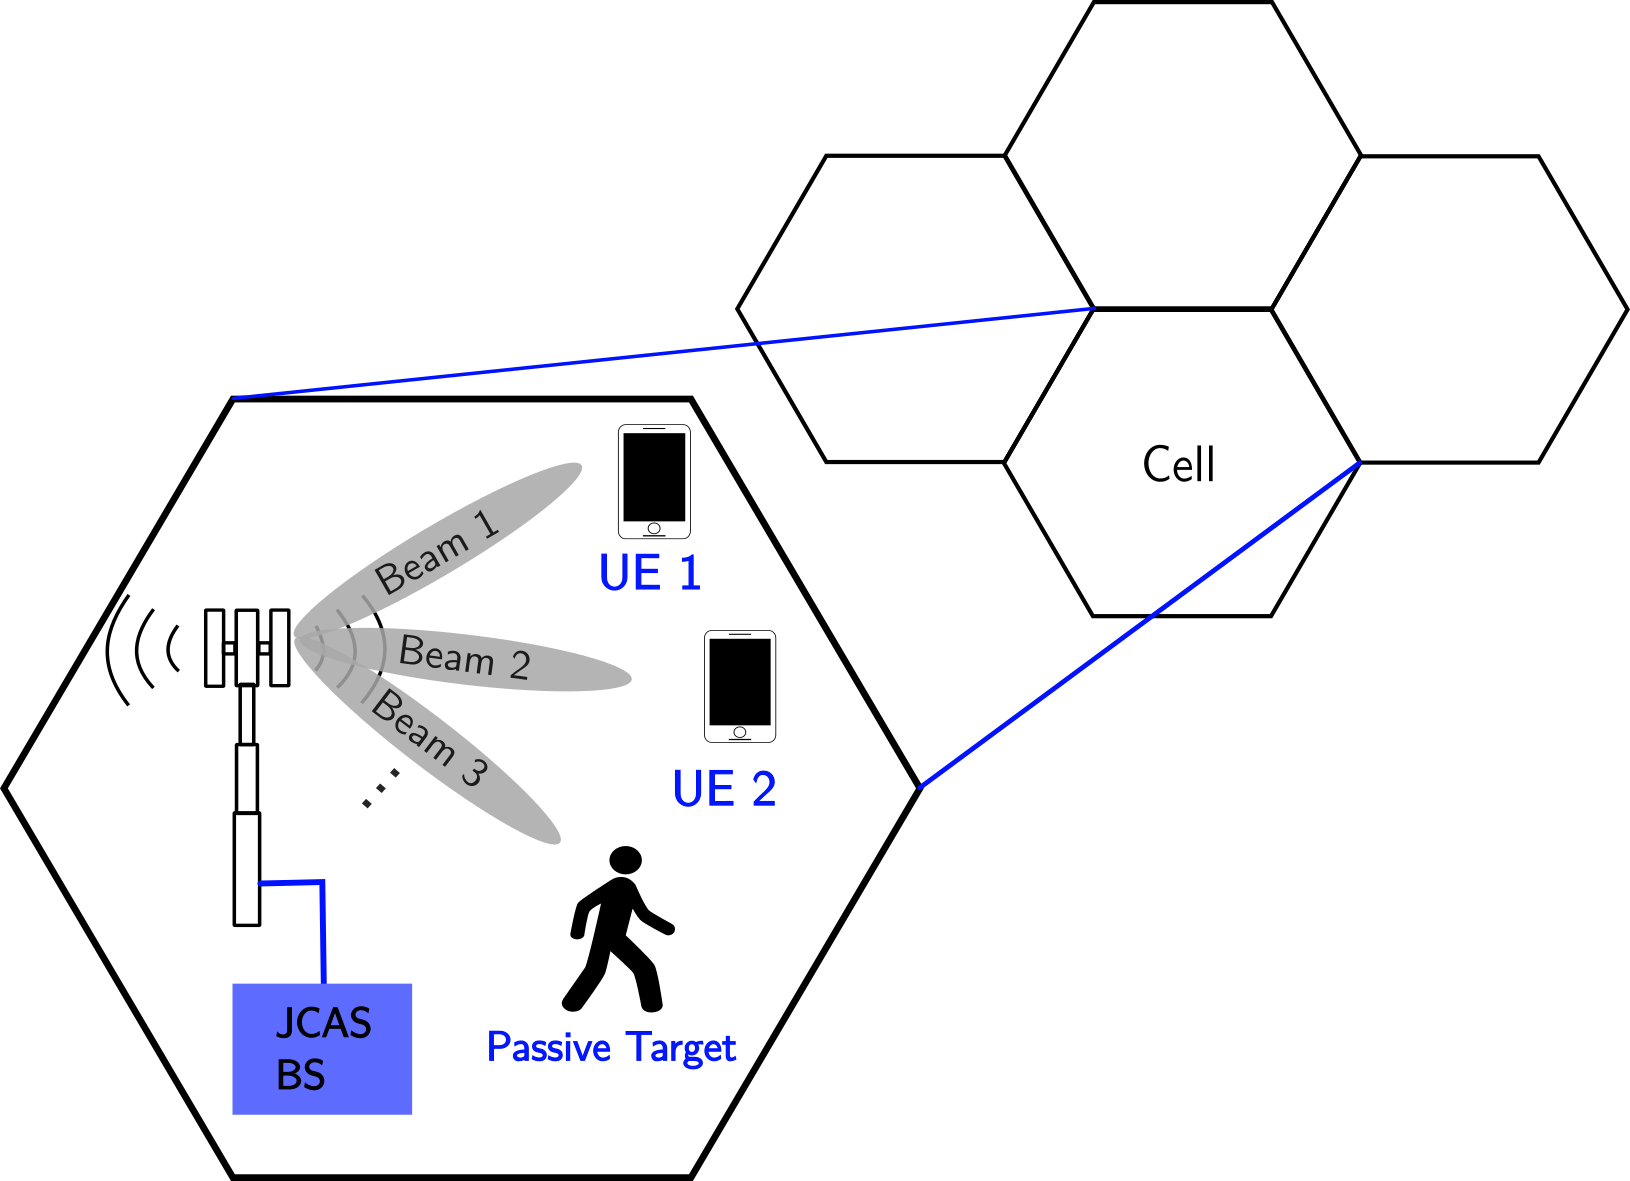
\includegraphics[width=0.7\textwidth]{Images/introduction/isac-scheme-1.png}
	\caption{Illustration of an ISAC scenario.}
	\label{fig:isac-scheme-1}
\end{figure}


Integrated sensing and communications will benefit from the current massive deployment of cellular systems and their increasing density: making use of existing hardware and extending its capabilities with sensing could enable multi-user communication and multi-target detection with extended coverage.



\section{Technological enablers}
	
	In recent years Radar and communication front-ends have become very similar, facilitating the integration of sensing and communication technology.
	Traditional radar systems were heavily reliant on hardware components to perform their core functions. However, with the advent of advanced digital technologies, a substantial number of these functions are now being realized through virtualization and digital signal processing. 

	This section will present some of the main technological aspects and digital technologies enabling joint functionality and the current research on radar in communication systems.	
	
	\subsection{Spectrum choice for 6G sensing}

	One of the goals set for the sixth generation of wireless networks is to make efficient usage of the available spectrum which is the scarcest resource in communications.
	
	Future systems will probably make use of larger frequency bands, exploiting high bandwidth to perform high-resolution sensing. From 20 MHz carriers in LTE, 100 MHz and 400 MHz in respectively 5G NR and mmWave NR, it can be expected that 5G evolution and 6G systems will use bandwidths in the order of 1 GHz or more. A large usable bandwidth allows for increased sensing resolution, comparable to the one of an ad-hoc radar systems.
	
	Spectrum choice will be the determinant factor for the definition of overall capabilities of the system. The frequency ranges that are being considered for 6G \cite{Hexa} are:
	
	\begin{itemize}
		\item Frequency Range 1 (FR1): from 600 MHz to 6 GHz;
		\item Frequency Range 2 (FR2): mmWave, from 24 GHz to 71 GHz;
		\item the new Frequency Range 3 (FR3), not yet specified: from 7 to 20 GHz
	\end{itemize}
	
	Frequency range 1 is currently used for 5G capacity layers, providing bandwidth up to 100 MHz. For 6G, the main capacity layer will be placed in the "Golden Band" in 6-14 GHz, offering up to 400 MHz of bandwidth. FR2 in the millimetre frequency bands will start at 24 GHz and offer significantly more bandwidth, up to 800 MHz.
	
	Golden Band and FR2 are the most relevant candidates for defining the sensing spectrum in 6G. Their selection would make sense for wide area sensing and high resolution sensing respectively.
	
	Feasible use cases and possible scenarios will be driven by the characteristics and specifications offered by the frequency band of choice. It can be expected that FR2 will be used in micro-cellular deployments. They will be deployed in indoor environments, such as factory floors. Sensing targets in such environment will likely be pedestrians, passive factory objects and vehicles.
	Macro-cellular environments in the Golden Bands will dominate outdoors, where targets of interest will e vehicles for traffic monitoring, roadside safety and even detection of unmanned aerial vehicles (UAV) or drones.
	
	\subsection{Waveform candidates for ISAC}
	
	Waveform design is a fundamental building block of any radar or communication systems. Traditional radar and communication systems use waveforms optimized for the respective use, that are, in general, very different \cite{Zhang_Rahman_Wu_Huang_Guo_Chen_Yuan_2022}.
	
	In this work we refer to a communication-centric design, where the communication system is adapted and expanded in order to perform the sensing operation, sharing the main hardware and resources provided by the wireless mobile network.
	 
	
	\subsubsection{Traditional radar waveforms}
	
	Conventional radar systems mainly consist of pulsed and continuous wave radar. Both types can be further categorised according to whether the wave is modulated in frequency or phase \cite{Friedlander_2007}.
	Pulsed radar transmits short, typically unmodulated, pulses or bursts of pulses of large bandwidth, followed by a silent period, waiting for the reception of the echoed signal. Continuos wave radar are currently largely used in the automotive systems and the main example is the frequency modulated continuous wave (FMCW) radar. This systems transmit chirp signals with fixed or variable frequencies, which get shifted by the so called beat frequency when they get reflected by objects.
	
	Radar systems are typically designed to enable high power transmission with a relatively simple receiver structure. Two of the main design objectives are amplifier efficiency and ideal autocorrelation properties of the radar wave. Waveforms with low peak-to-average power ratio (PAPR) enable high efficiency and long range transmission.
	
	Due to their specialized signal shape and relatively simple hardware, this systems cannot support high data-rates for communication purposes, especially the ones that will be required by 6G.
	
	\subsubsection{Communication-centric waveforms}
	
	Current mobile communications are dominated by single-carrier and multi-carrier waveforms (OFDM).
	OFDM has become the current waveform reference in ISAC. Fully established in 4G and 5G communications systems, in the last decade it has also attracted the attention of the radar world.
	
	OFDM offers great multiplexing capabilities, both in time and in frequency, through the definition \textit{OFDM resource elements} that can be dynamically allocated to users. The use of cyclic prefix transforms the linear convolution of the signal with the channel response into a circular convolution, allowing convenient equalisation of the channel in the frequency domain \cite{Wild_Grudnitsky_Mandelli_Henninger_Guan_Schaich_2023}. In scenarios limited by PAPR constraints, such as uplink transmission, DFT spreading can  be applied on top of OFDM to achieve a single-carrier frequency division multiple access (SC-FDMA) scheme.
	
	Multicarrier waveforms offer the possibility of obtaining sensor information by using signal processing techniques that reduce the autocorrelation requirements required to radar waveforms \cite{Sturm_Wiesbeck_2011}.The main disadvantage of OFDM is the high peak to average power ratio (PAPR) and the additional DSP required for the joint communication and sensing data processing.
	
	\subsubsection{Waveforms for next-gen communication networks}
	
	A major challenge for OFDM and multi-carrier signals is their performance in highly frequency-dispersive channels. 
	The effect of phase noise and movement (Doppler spread) is enhanced at high carrier frequencies. 
	Due to the expansion of 5G and 6G systems towards mmWave, tackling this challenge is fundamental for ensuring high performance under these circumstances.
	
	Orthogonal time frequency space (OTFS) has been proposed as a modulation effective in tackling this problems \cite{OTFS_Hadani_2017}. OTFS operates in the delay-Doppler domain. 
	The fading, time-variant channel seen by an OFDM signal is transformed into a non-fading, time-independent channel through a 2D Fourier transform. 
	Applying this transformation and equalization within this domain each symbol will experience similar gain during transmission.
	
	The Orthogonal Time Frequency Space (OTFS) modulation scheme can be interpreted as the sequence of two transformations. 
	Firstly, the transmitter maps the complex symbols into discrete slots of the NxM delay-Doppler domain.
	Secondly, these symbols are transformed in the time-frequency domain through a 2D inverse symplectic finite Fourier transform (iSFFT). The the time-domain signal is obtained by an M-point inverse Fourier transform (iFFT). 
	The receiver will perform the inverse operation using FFT and SFFT respectively.
	OTFS is an ideal waveform for integrating sensing and communication due to its inherent property of exploiting the delay-Doppler domain.
	This is because information about the surrounding environment is necessary for improving communication performance.
	
	Although OTFS has proved to achieve a 3-7 dB advantage compared to OFDM in highly fading and mobility scenarios, however its implementation in real systems is hindered by some open research problems \cite{Wei_Yuan_OTFS_whitepaper_2021}. 
	The primary challenge is to develop an efficient decoding method for OTFS symbols.
	The output signal in the delay-Doppler domain is 2D circular convolution of the transmitted data symbols and the channel response. Although optimal detectors, such as maximum a posteriori (MAP) detectors, can mitigate channel interference and perfectly retrieve the original symbols, but they are too complex and costly.
	
	This work will focus on Orthogonal Frequency Division Multiplexing (OFDM), as it is the waveform currently used in 5G systems and in the proof of concept by Nokia. 
	
	 
	
	\subsection{5G functional splits}
	
	A functional split determines the number of functions implemented locally at the antenna site and, consequently, the functions to be implemented in a centralised datacenter \cite{Larsen_Checko_Christiansen_2019}. 
 	This solution was developed to define a flexible approach to the centralised radio access network (C-RAN) concept, that could work with the high data rates expected in 5G. 
	In NR, the radio processing stack defined by 3GPP is split between a distributed unit (DU) and a centralised unit (CU). 
	The general idea is to keep functions close to the user in the DU, while placing more complex and computationally intensive functions in the CU. The CU is usually represented by powerful datacenters.
	Allocating more functions in the DU means less traffic on the fronthaul network, but requires more powerful and expensive hardware at the antenna site.
	 
	Functional splits allow for a fairly flexible architecture of the system. Additional functionality, such as network sensing, can be implemented at the antenna site by adding dedicated processing hardware.

	\begin{figure}[H]
		\centering
		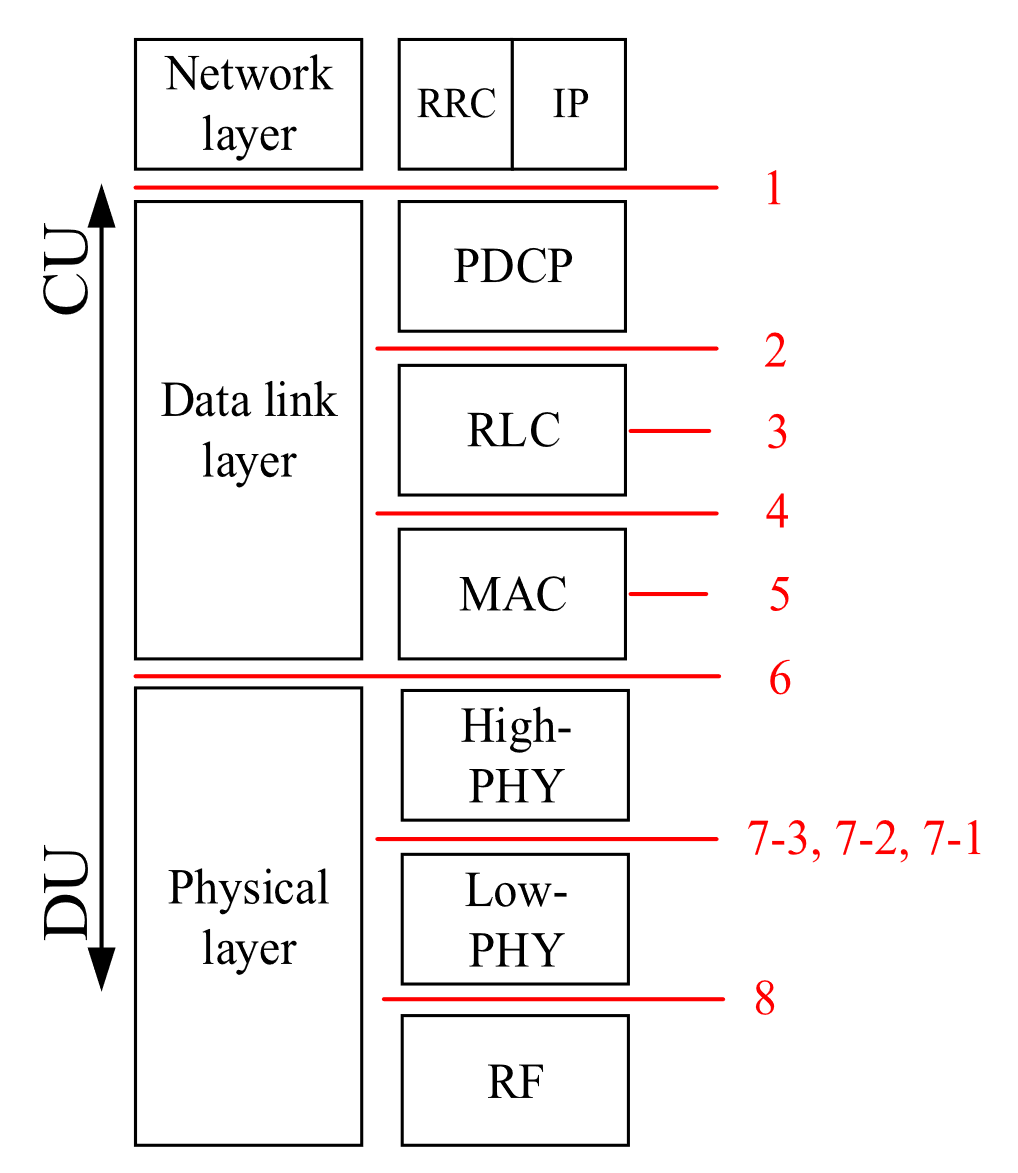
\includegraphics[width=0.5\textwidth]{Images/overview/5Gsplits_Larsen.png}
		\caption{Scheme representing the LTE protocol stack, showing proposed functional splits \cite{Larsen_Checko_Christiansen_2019}. }
		\label{fig:Overview-LTE_stack_splits}
	\end{figure}
	 
	
	\subsection{Massive MIMO and digital beamforming}
	
	Massive MIMO and digital beamforming can set the basis for performing high-resolution three-dimensional scans of the surrounding environment \cite{MIMO-next-gen}.
	The general idea is to intelligently combine the signals received from multiple antennas to achieve the best signal-to-noise ratio and the highest data rate. The signal combination is performed in the digital domain, after conversion to baseband, which offers the possibility of applying a variety of algorithms.
	
	In 5G, beamforming commonly employs an all-digital approach at lower frequencies. However, for mmWave frequencies and above, digitally controlled analogue or hybrid beamforming is typically used. In the hybrid approach one beam gets scanned at a time. A beam sweep can be performed by the transmitting cells, and the procedure of computing the range-Doppler profile of all beams in a cell is referred to as beam sweep. A similar procedure to a beam sweep is already used in 5G NR for synchronization signalling \cite{Wild_Braun_Viswanathan_2021}.
	
	\subsection{Signal processing enhanced by AI/ML}
	Generally, radar returns provide additional information beyond the range-Doppler profile. 
	By analysing the channel information, it may be possible to extract target characteristics such as radar cross-section, micro-Doppler information, or the object's material or shape.
	This additional information can be used to solve a classification problem of objects and returns detected in the radar datacube (target information represented in the range-Doppler-angular domain).
	
	Recent years have seen AI/ML emerging as a novel and powerful method for extracting and processing information effectively, often surpassing traditional methods.
	In the radar world AI has been used to solve target classification problems. 
	AI systems can accurately differentiate between various targets, such as aircraft, ships, and ground vehicles, based on their radar signatures. 
	AI-powered radar systems can adapt and learn from new data, continuously improving their capabilities over time. 
	This technology could assist the development of autonomous radar systems capable of making independent decisions based on the classification results. 
	
	 Furthermore, artificial intelligence and machine learning have been introduced in communication systems to optimize network resources, improve overall quality of service, solve optimization problems, and predict system load and traffic. 
	 By combining sensing capabilities with artificial intelligence (AI), nodes could effortlessly integrate the physical and digital domains, giving the network situational capabilities.
	


\section{Proof of concept architecture}
	\label{sec:intro-PoCarchitecture}
	
	One of the objectives of ISAC is to make the best use of the deployed communication hardware to perform sensing. 
	The architecture considered in this work is based on a FR2 5G commercial communication hardware.
	
	Using option 7-2 of the proposed 5G splits, shown in Figure \ref{fig:Overview-LTE_stack_splits}, it is possible to use the same type of Remote Unit (RU) for both communication and sensing.
	Option 7-2 splits the network at the physical layer (PHY) level, which handles the conversion of digital data to the analogue radio signal in the downlink (DL) direction, while doing the opposite in the uplink (UL) direction.
	This split defines the FFT/iFFT performed in the RU, while the frequency domain IQ is transported on the fronthaul.
	The gNB RU operates in time-division duplexing (TDD) mode, where uplink is separated from downlink by the allocation of different time slots in the same frequency band. 	
	The sniffer operates always in uplink (UL) mode, receiving both the signal transmitted by UEs and the reflected signals. 
	
	The system is extended by an additional RU called \textit{Sniffer} and a server called \textit{Sensing Processing Unit} (SPU). 
	The sniffer is synchronized with the gNB by the same synchronization source. 
	The SPU receives the complex IQ signal (on a per-radio frame basis),  after removal of the cyclic prefix (CP), as input for further sensing processing \cite{Wild_Grudnitsky_Mandelli_Henninger_Guan_Schaich_2023}.
	
	This work considers a PoC deployment where the primary gNB RU and the sniffer are mounted in proximity and are co-located, allowing the system to behave as a monostatic radar. 
	The scope of this work does not cover the case of bistatic radar.
	
	The SPU processing chain for sensing is structured as follows:
	
	\begin{itemize}
		\item \textit{Reference and reflected signal reception}. Receive and process packets from gNB and Sniffer. Each radio frame has dimension NxM, where N is the number of subcarriers and M the number of OFDM symbols.
		\item \textit{Channel computation}. Channel information is obtained by performing element-wise division between received and transmitted frames.
		\item \textit{Clutter removal}. Before every measurement, the channel of the corresponding scenario without targets is saved during a calibration step and it is subtracted from the reflected signal at runtime.
		\item \textit{Periodogram computation}. The spectral response of the channel information is obtained by computing N FFTs followed by M iFFTs on the result. The response is then converted in a 2D Range-Doppler map of the observed targets. 
		\item \textit{Peak extraction}. Identifying the peaks in the periodogram allows to retrieve the range-speed information of targets present on the scene.
		\item \textit{Target tracking}. A Kalman Filter (KF) can be used to track the detected targets. 
	\end{itemize} 
	A more detailed description on how the processing chain is structured,  based on \cite{Braun2014OFDMRA}, will be presented in Chapter \ref{chap:theoretical_OFDM}.
	
	
	\subsection{System parameters}
	
	The system specifications are indicated in table \ref{table:PoCparams}.They correspond to parameters for 5G NR systems with the numerology $\mu=3$. \cite{TS138211}. 
	
	\begin{table}[H]
		%\caption*{\textbf{Title of Table (optional)}}
		\centering 
		\begin{tabular}{|p{9em} c c |}
			\hline
			\rowcolor{bluepoli!40} % comment this line to remove the color
			\textbf{Parameter} & \textbf{Description} & \textbf{Value}  \T\B \\
			\hline \hline
			$\bm{\mu}$ & 5G numerology & 3 \T\B \\
			$\bm{f_C}$ & carrier frequency & 27,4 GHz \T\B \\
			$\bm{B}$ & bandwidth & 200 MHz \T\B\\
			$\bm{\Delta_f}$ & subcarrier spacing & 120 kHz  \T\B\\
			$\bm{T_S = 1/\Delta_f + T_{CP}}$ & symbol time & 8,923 $\mu s$  \T\B\\
			$\bm{T_{CP}}$ & cyclic prefix time & 0,59 $\mu s$  \T\B\\
			$\bm{N}$ & number of subcarriers & 1584  \T\B\\
			$\bm{M}$ & number of symbols & 1120  \B\\
			
			\hline
		\end{tabular}
		\\[10pt]
		\caption{List of system parameters from NOKIA proof of concept installation.}
		\label{table:PoCparams}
	\end{table}
	
	The system is equipped with analog beamforming and measurements can be obtained using a fixed beam chosen by an antenna codebook.


\section{Sensing use-cases}

	A number of use-cases has been proposed \cite{Mandelli_Henninger_Bauhofer_Wild_2023}, \cite{Wang_Varshney_Gentile_Blandino_Chuang_Golmie_2022} and some of the  key requirements for each application have been estimated in \cite{Wild_Braun_Viswanathan_2021}.
	
	Defining probable scenarios and use cases for ISAC 
	
	% TODO
	...
	\alert{FINIREEEE BUONFIORNOOOOO KAFFE?}
	\subsection{Vehicle activities}
	
	\subsection{Human activities}
	
	\subsection{Weather sensing}
	
	\subsection{Non-line-of-sight sensing}
	
	The term \textit{line-of-sight} (LOS)  denotes the existence of a direct, unobstructed line of sight between the transmitter and the target. On the contrary, \textit{non-line-of-sight} (NLOS) denotes the condition in which the target is reached by the transmitted signal by reflection on another entity.
	
	This work explores the potential feasibility of non-line-of-sight sensing and its possible use cases in ISAC.
	
	Non-line-of-sight sensing has a significant advantage in achieving 'around the corner' detection, which is not feasible with traditional fixed camera or LIDAR systems. Advanced sensing techniques and algorithms can enable non-line-of-sight systems to detect and track objects or individuals even when direct line-of-sight visibility is obstructed.
	
	In addition, non-line-of-sight sensing has the potential to enhance cellular sensing systems in a cost-effective manner, making them a viable alternative to expensive ad hoc systems. This approach does not require the deployment of infrastructure or specialized equipment. Early explorations of non-line-of-sight sensing suggest that it is possible to leverage existing network hardware and extend its capabilities. Non-line-of-sight sensing could be an attractive option for industries seeking to enhance their surveillance or monitoring systems while optimizing resources.
	
	Furthermore, it could unlock new use cases that have yet to be fully explored. In industrial environments, non-line-of-sight sensing technology has the potential to enhance safety protocols and improve accident prevention measures by detecting humans within obscured or complex settings. Additionally, intrusion detection systems could benefit from this technology as it may enable the identification of unauthorized access attempts even in hidden or non-obvious entry points.
	
	This work focuses on intrusion detection in industrial scenarios as the primary working scenario of the system. 
	
	

